\section{Verklarende Macro-Economie}

In de \textit{beschrijvende} \entry{macro-economie} definieerden we een aantal concepten en gaven we een aantal cijfers om die concepten te illustreren. We gaan nu over tot de \textit{verklarende} \entry{macro-economie}, waar we een onderscheid maken tussen de aanbodzijde en de vraagzijde.\\

\par Hernemen we even het concept van het potentieel \entrystyled{bbp}{BBP} (hoofdstuk \ref{sec:h5groei}). Het potentieel BBP gaat over de \term{aanbodcapaciteit} ; hoeveel arbeid men over beschikt, over hoeveel kapitaalstock men heeft, en wat de technologie\"en zijn die men met deze kapitaalstock samen kunnen gebruiken.
\par De feitelijke productie hangt af van \textit{vraagschommelingen}. Die kunnen het gevolg zijn van externe schokken, zoals bij de terroristische aanval in Zaventem.
\par Het verschil tussen het potentieel - en feitelijk BBP (dat van Belgi\"e wordt weergegeven in figuur \ref{fig:h6bbpbelgie}) zorgt voor een outputkloof.\\

\begin{figure}[H]
\small\centering\captionsetup{justification=centering,margin=2cm}
\begin{tikzpicture}
\begin{axis}[scaled y ticks=false,axis lines=left,axis line style=gray,/pgf/number format/.cd, use comma, width=0.5\linewidth, legend cell align=left,legend style={at={(axis cs:1860,15000)},anchor=south west,draw=none},ymin=0,ymax=35000]
\addplot[blue] table [x=Jaar Geobserveerd, y=Geobserveerd, col sep=comma] {Data/H6-BelgieBBP.csv};
\addplot[red] table [x=Jaar Constante, y=Constante, col sep=comma] {Data/H6-BelgieBBP.csv};
\addlegendentry{Feitelijk BBP}
\addlegendentry{Potentieel BBP}
\end{axis}
\end{tikzpicture}
\caption{Het Belgisch BBP per capita}
\label{fig:h6bbpbelgie}
\end{figure}

\par In wat volgt maken we abstractie van de invloed van de aggregatieve vraag (alle bestedingen samengenomen). We maken dus abstractie van het bestaan van een \entry{outputkloof} en daarom ook van \entry{conjuncturele werkloosheid}\footnote{Er is sprake van conjuncturele werkloosheid als de werkloosheid groter is dan de \entry{natuurlijke werkloosheid}. Dan is er een negatieve \entry{outputkloof}.}.\\

\par\noindent Hernemen we even de formule in hoofdstuk \ref{sec:h1prod} :
$$\frac{BBP_n}{\text{bevolking}}=\frac{BBP_n}{Tew_n}\cdot\frac{Tew_n}{\text{beroepsbevolking}}\cdot\frac{\text{beroepsbevolking}}{\text{\#15-65-jarigen}}\cdot\frac{\text{\#15-65-jarigen}}{\text{bevolking}}$$
Hier met $BBP_n$ het natuurlijke of potentiele \entrystyled{bbp}{BBP}, en $Tew_n$ de natuurlijke tewerkstelling (`\textit{natuurlijke}' omdat er abstractie wordt gemaakt van conjunctuurschommelingen).
Zoals men eerder opgemerkte is de derde factor de \entry{participatiegraad} of de \entry{activiteitsgraad}. De tweede factor is de \entry{werkgelegenheidsgraad} of \entry{werkzaamheidsgraad}. De eerste factor is de \entry{arbeidsproductiviteit}.
\par De \entry{werkloosheidsgraad} is uiteraard gelijk aan 100\% minus de werkgelegenheidsgraad (in procent).
\par Al deze begrippen zullen van belang zijn in wat volgt ...\\

\subsection{Arbeidsaanbod}

\subsubsection{Volmaakte Mededinging - De Activiteitsgraad}

\textit{Hoe komt het dat wij een re\"eel loon hebben dat 30 keer zo groot is dan dat in Burkina Faso, en 20 keer zo groot als dat van onze voorouders?}  Dat komt door  de \entry{arbeidsproductiviteit}. En het komt zeer goed tot uiting in de \entry{volmaakte mededinging}. De hypothese van volmaakte mededinging is onrealistisch, maar biedt ons wel inzicht in het re\"ele loon, in de scholingspremie, en in de invloed van werknemers- en werkgeversbijdragen op de \entry{activiteitsgraad}.
\par Maar de hypothese biedt ons helaas geen inzicht in de invloed van onderhandelingen en van de heterogeniteit van de arbeid, en het is onder andere hierdoor dat de werkloosheid `\textit{weggedacht}' wordt.

\paragraph{Het evenwichtsloon}

Arbeid wordt gevraagd door werkgevers en aangeboden door werknemers en zelfstandigen. De parti\"ele vraagfunctie van de werkgevers ziet er zo uit :
$$Q_a^v=f(\frac{w}{P}\ |\ \text{\#bedrijven, technologie, ...})\quad\text{ (met }w\text{ het \term{nominaal loon}, }P\text{ een prijsindex, en }\frac{w}{P}\text{ het re\"eel loon)}$$
De prijsindex is de prijs van een representatieve korf goederen. \\
We kijken dus naar het re\"eel loon en diens invloed op de vraag naar arbeid, waarbij alle andere omstandigheden (zoals het aantal bedrijven) gelijk blijven (\entry{ceteris paribus}). Deze invloed is \textit{negatief}.

\par\noindent De parti\"ele aanbodfunctie van de werknemers ziet er dan weer zo uit :
$$Q_a^a=g(\frac{w}{P}\ |\ \text{pref, NAI, POP, ...})\quad\text{ (met }w\text{ het \term{nominaal loon}, }P\text{ een prijsindex, en }\frac{w}{P}\text{ het re\"eel loon)}$$
Deze keer is de invloed van het re\"eel loon \textit{positief} : hoe hoger, hoe meer vraag er gaat zijn.\\

\par Wat steekt er `\textit{achter}' de vraagcurve? Zoals altijd is dat de marginale betalingsbereidheid voor arbeid. En die valt samen met de marginale arbeidsproductiviteit, die daalt met de hoeveelheid arbeid. Als je bijvoorbeeld een veld laat bewerken, dan gaat de eerste arbeider veel werk kunnen leveren, maar als er meer arbeiders bijkomen, dan zal de gewonnen productiviteit zal zijn. Als er z\'e\'er veel arbeiders bijkomen zou het zelfs kunnen dat ze elkaar verhinderen.
\par Wat steekt er `\textit{achter}' de aanbodcurve? De marginale kost van de arbeid. Aan arbeid verliest een mens vrije tijd. Wij appreci\"eren vrije tijd. En hoe meer men die vrije tijd opgeeft, hoe zeldzamer ie wordt, en hoe meer waarde men eraan hecht. De marginale kost (de opportuniteitskost) valt samen met de marginale betalingsbereidheid voor vrije tijd en stijgt dus met de hoeveelheid arbeid.
\par Als de bevolking groter wordt, dan schuift de aanbodcurve naar rechts. Wordt de bevolking kleiner\footnote{Bij het uitbreken van de pest was er bijvoorbeeld een scherpe daling van de bevolking en gingen de lonen omhoog.}, dan schuift hij naar links.\\

\par Figuur \ref{fig:h6arbeideven} illustreert het evenwicht bij gegeven vraag- en aanbodcurve. Dat ontstaat waar de marginale betalingsbereidheid gelijk is aan de marginale productiviteit van arbeid. Als we werkloosheid defini\"eren als een situatie waarbij mensen die zouden willen werken aan het gegeven loon geen werk vinden, dan kan het model van perfecte concurrentie op de arbeidsmarkt werkloosheid niet verklaren.

\begin{figure}[H]
\vspace{0.5cm}
\centering\small
\captionsetup{justification=centering,margin=2cm}
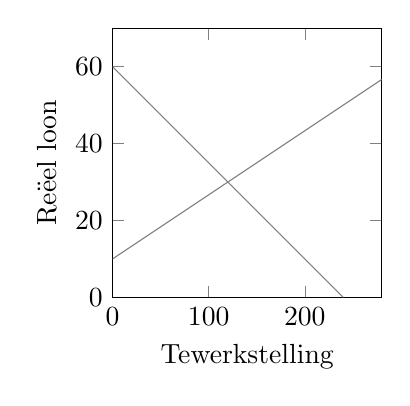
\begin{tikzpicture}
	\begin{axis}[name=left,xlabel=Tewerkstelling, ylabel={Re\"eel loon}, ymin=0, xmin=0, xmax=280, ymax=70,width=5cm, height=5cm]
		\addplot[gray, samples=120, domain=0:280] {10+(1/6)*x};
		\addplot[gray, samples=120, domain=0:240] {60-(1/4)*x};
	\end{axis}
\end{tikzpicture}
\caption{Het evenwicht op de arbeidsmarkt}
\label{fig:h6arbeideven}
\end{figure}

Dit voorbeeld ligt veraf van de dagelijkse werkelijkheid, maar leert ons dat het re\"ele loon gelijk is aan de arbeidsproductiviteit, en dat als we op de lange termijn loonstijgingen krijgen, dat dat de maken heeft met de stijging van de arbeidsproductiviteit.
\par Stijging van het \entrystyled{bbp}{BBP} (het loon) komt dus door de stijging van de arbeidsproductiviteit (waardoor de vraagcurve naar rechts schuift). Zo'n stijging wordt veroorzaakt door investeringen in machines (stijging van de \entry{kapitaalstock}) en in technologische vooruitgang.
\par Zoals men al eerder opmerkte kan het re\"eel loon ook stijgen omdat de aanbodcurve naar links verschuift, zoals bij een catastrofe die de bevolking doet dalen.\\

\paragraph{De scholingspremie}

De \entry{scholingspremie} is het extra loon dat je krijgt omdat je langer gestudeerd hebt. In Chili is deze zeer groot : zij die hoger onderwijs achter de rug hebben, verdienen meer dan 2,5 keer zo veel als zij die enkel hun middelbaar diploma hebben. In Belgi\"e is het verschil heel wat kleiner, daar verdienen mensen met een diploma hoger onderwijs zo'n 25\% meer.
\par De reden waarom het verschil tussen lage lonen en toplonen toeneemt is de stijging van de scholingspremie. Deze stijging heeft te maken met vraag en aanbod naar geschoolde arbeid. \\

\par In figuur \ref{fig:h6schoolarbeid} geeft men de koers tussen de technologische vooruitgang en de democratisering van het onderwijs weer. De technologische vooruitgang bepaalt de vraag naar geschoolde arbeid\footnote{In deze context kan opgemerkt worden dat het vooral de middenklasse is die er aan verliest. Bepaalde jobs zoals poetsen worden immers niet bedreigd door machines, en daar is dan meer vraag naar.}, en de democratisering van het onderwijs verklaart het aanbod van geschoolde arbeid.
\par De grafiek geeft de \textit{relatieve} vraag (of relatief aanbod) weer, dat wil zeggen, de verhouding van de vraag naar hooggeschoolden naar die van laaggeschoolden. Technologische vooruitgang doet de vraag naar rechts en naar boven verschuiven, omdat de vraag verhoogt en de werkgevers bereid zijn om meer te betalen.

\begin{figure}[H]
\vspace{0.5cm}
\centering\small
\captionsetup{justification=centering,margin=2cm}
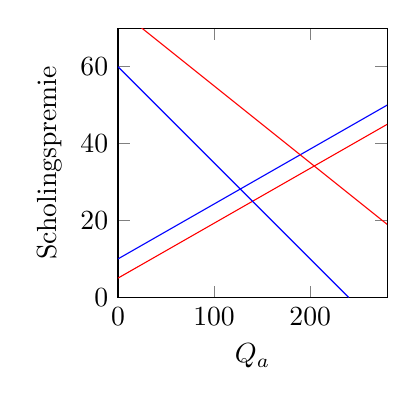
\begin{tikzpicture}
	\begin{axis}[name=left,xlabel={$Q_a$}, ylabel={Scholingspremie}, ymin=0, xmin=0, xmax=280, ymax=70,width=5cm, height=5cm]
		\addplot[blue, samples=120, domain=0:280] {10+(1/7)*x};
		\addplot[red, samples=50, domain=0:280] {5+(1/7)*x};
		\addplot[red, samples=120, domain=0:280] {75-(1/5)*x};
		\addplot[blue, samples=50, domain=0:240] {60-(1/4)*x};
	\end{axis}
\end{tikzpicture}
\caption{Effect technologische vooruitgang en democratisering van het onderwijs op scholingspremie}
\label{fig:h6schoolarbeid}
\end{figure}

\noindent De \entry{globalisering} zorgt er ook voor dat er meer vraag naar hooggeschoolden is ; terwijl laaggeschoolden competitie moeten ondervinden door de verplaatsing (\term{offshoring}) van werk, profiteren de hooggeschoolden van de globalisering omdat zij hun capaciteiten in zekere zin op de wereldmarkt te gelde kunnen maken.\\

\par De loonwaaier wordt gedeeltelijk verklaard door de \entry{scholingspremie}, maar er zijn een aantal anomalie\"en die er niet verklaard door kunnen worden. Als je immers kijkt naar de top 10\% lonen, de top 1\%, de top 0.1\%, ... dan is er daar enorme ongelijkheid\footnote{We verwezen eerder al naar Thomas Piketty, die het hierover heeft.}. En toch hebben deze mensen allemaal hetzelfde diploma. In Zuid-Afrika is de loonwaaier minder breed dan in de Verenigde Staten. 
\par Er zijn dus andere factoren aan het werk dan enkel de technologische vooruitgang en de democratisering van het onderwijs. E\'en factor is de aanwezigheid van instituties. Zo zijn er onderaan de loonladder \textbf{minimumlonen}\index{minimumloon} (zie figuur \ref{fig:h6minimum}) en onderhandelende loonbarema's. Bovenaan de loonladder worden toplonen bepaald via vriendelijke remuneratiecomit\'es, waardoor men grosso modo de eigen loon kiest. Daar zijn er ook veranderingen van normen, zoals bij de hoge lonen van voetballers.

\begin{figure}[H]
\small\centering\captionsetup{justification=centering,margin=2cm}
\begin{tikzpicture}
\begin{axis}[scaled y ticks=false,axis lines=left,axis line style=gray,/pgf/number format/.cd, use comma, width=0.5\linewidth, legend cell align=left,legend style={at={(axis cs:1975,1)},anchor=south west,draw=none},ymin=0,ymax=10]
\addplot[blue] table [x=Jaar, y=Frankrijk, col sep=comma] {Data/H6-MinimumLoon.csv};
\addplot[red] table [x=Jaar, y={Verenigde Staten}, col sep=comma] {Data/H6-MinimumLoon.csv};
\addlegendentry{Frankrijk}
\addlegendentry{Verenigde Staten}
\end{axis}
\end{tikzpicture}
\caption{Minimumlonen in Frankrijk en de Verenigde Staten}
\label{fig:h6minimum}
\end{figure}

\begin{figure}[H]
\small\centering\captionsetup{justification=centering,margin=2cm}
\begin{tikzpicture}
\begin{axis}[scaled y ticks=false,axis lines=left,axis line style=gray,/pgf/number format/.cd, use comma, width=0.5\linewidth, legend cell align=left,legend style={at={(axis cs:1915,-0.018)},anchor=south west,draw=none},ymin=-0.02,ymax=0.24,ytick={0,0.02,0.04,0.06,0.08,0.10,0.12,0.14,0.16,0.18,0.20,0.22,0.24},yticklabels={0\%,2\%,4\%,6\%,8\%,10\%,12\%,14\%,16\%,18\%,20\%,22\%,24\%}]
\addplot[blue] table [x=Jaar, y=Centiel2, col sep=comma] {Data/H6-Centiel.csv};
\addplot[red] table [x=Jaar, y={Zonder Meerwaarden}, col sep=comma] {Data/H6-Centiel.csv};
\addplot[gray] table [x=Jaar, y=Centiel, col sep=comma] {Data/H6-Centiel.csv};
\addlegendentry{Aandeel bovenste centiel nationaal inkomen}
\addlegendentry{Zonder meerwaarden}
\addlegendentry{Loonaandeel bovenste centiel}
\end{axis}
\end{tikzpicture}
\caption{Evolutie van bovenste centiel van de bevolking in de Verenigde Staten}
\label{fig:h6centiel}
\end{figure}

\paragraph{Sociale bijdragen}

Sociale bijdragen zijn een soort \entry{belasting} die op de werkgevers of werknemers toegepast kunnen worden. Het is een belasting langs beide zijden van de markt. Dit be\"invloed de vraag- en aanbodcurve. Als de werkgevers naast een salaris aan werknemers ook nog bijdragen moeten betalen, dan gaat de vraagcurve naar links verschuiven. Als de werknemers een deel van hun salaris moeten afstaan, dan gaat de aanbodcurve ook naar links verschuiven. De \entry{activiteitsgraad} daalt.\\

\par We illustreren dit even met een voorbeeld in figuur \ref{fig:h6bijdragen}. Het \entry{brutoloon} is het loon dat de werkgever betaalt aan de werknemer. Het \entry{nettoloon} is het brutoloon waarvan de sociale bijdragen zijn afgetrokken. De \entry{loonkosten} zijn de som van het brutoloon en de werkgeversbijdragen. En de \entry{loonwig} is het verschil tussen de loonkosten en het nettoloon dat de werknemer ontvangt. In Belgi\"e was de loonwig 53\%.
\par De wig verkleinen kan via een \term{taxshift} (zoals de Turteltaks).

\begin{figure}[H]
\vspace{0.5cm}
\centering\small
\captionsetup{justification=centering,margin=2cm}
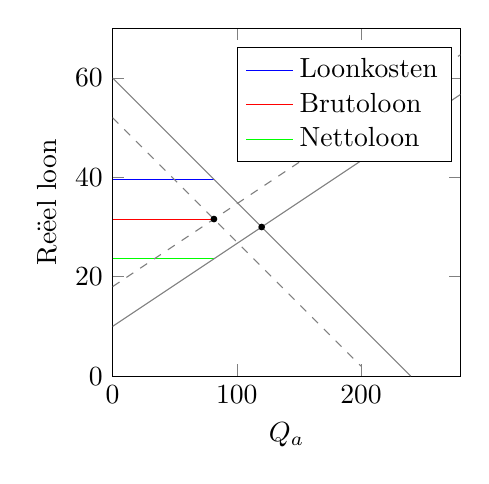
\begin{tikzpicture}
	\begin{axis}[name=left, legend cell align=left,legend style={at={(axis cs:100,43)},anchor=south west},xlabel={$Q_a$}, ylabel={Re\"eel loon}, ymin=0, xmin=0, xmax=280, ymax=70,width=6cm, height=6cm]
		\addplot[blue] coordinates {(0,39.6) (81.6,39.6)};
		\addplot[red] coordinates {(0,31.6) (81.6,31.6)};
		\addplot[green] coordinates {(0,23.6) (81.6,23.6)};
		\addplot[gray, samples=50, domain=0:280] {10+(1/6)*x};
		\addplot[gray, samples=50, domain=0:240] {60-(1/4)*x};
		\addplot[gray, dashed, samples=50, domain=0:280] {18+(1/6)*x};
		\addplot[gray, dashed, samples=50, domain=0:200] {52-(1/4)*x};
		\node[label=above:{},minimum size=2pt, fill=black, inner sep=0pt, shape=circle, draw] at (axis cs:120,30) {};
		\node[label=above:{},minimum size=2pt, fill=black, inner sep=0pt, shape=circle, draw] at (axis cs:81.6,31.6) {};
		\addlegendentry{Loonkosten}
		\addlegendentry{Brutoloon}
		\addlegendentry{Nettoloon}
	\end{axis}
\end{tikzpicture}
\caption{Sociale bijdragen en de daling van de activiteitsgraad}
\label{fig:h6bijdragen}
\end{figure}

\subsubsection{De Natuurlijke Werkloosheid en de Natuurlijke Tewerkstelling}

De \entry{natuurlijke werkloosheid} is die werkloosheid die zorgt voor een constante \entry{inflatie}. Om die reden gebruikt men de afkorting \textit{NAIRU}\footnote{Ge\"introduceerd door Milton Friedman.} : `\textit{Non-Accelerating Inflation Rate of Unemployment}'. Het is dus de werkloosheid die ervoor zorgt dat de inflatie constant blijft. Het is de werkloosheid die blijft bestaan, zelfs al draait de economie op volle toeren. Men kan ze niet elimineren. Vakbonden horen er dus niet graag van.\\

\par In figuur \ref{fig:h6werkloosheid} wordt de natuurlijke werkloosheid weergegeven naast de feitelijke werkloosheid. Als deze hoger ligt, dan is dit door de \entry{conjuncturele werkloosheid}. Als hij lager ligt, dan is dit door \entry{inflatoire druk} : de inflatie versnelt.

\begin{figure}[H]
\small\centering\captionsetup{justification=centering,margin=2cm}
\begin{tikzpicture}
\begin{axis}[scaled y ticks=false,axis lines=left,axis line style=gray,/pgf/number format/.cd, use comma, width=0.4\linewidth, legend cell align=left,legend style={at={(axis cs:1990,2)},anchor=south west,draw=none}]
\addplot[blue] table [x=Jaar, y=Natuurlijke, col sep=comma] {Data/H6-Werkloosheid.csv};
\addplot[red] table [x=Jaar2, y=Feitelijke, col sep=comma] {Data/H6-Werkloosheid.csv};
\addlegendentry{Natuurlijke}
\addlegendentry{Feitelijke}
\end{axis}
\end{tikzpicture}
\caption{Evolutie van bovenste centiel van de bevolking in de Verenigde Staten}
\label{fig:h6werkloosheid}
\end{figure}

\paragraph{Loonstarheid}

\paragraph{De Heterogeniteit van Arbeid}